\documentclass[12pt,a4paper]{article}
%le préambule

\usepackage[T1]{fontenc}
\usepackage[francais]{babel}
\usepackage{url} % permet l'utilisation de la balise url pour les liens internet
\usepackage{graphicx} % permet l'utilisation des images

\title{Rapport Projet Dev Web} % titre de l'article
\author{GIRAUD Nicolas // COURT Anthony} % auteur de l'article
\date{18 Mai 2025} % date de l'article

%document principal
\begin{document}

\maketitle
\newpage

\tableofcontents
\newpage

\section{Présentation Générale}
\subsection{En quoi consiste notre projet?}
Pour ce projet nous avons décider de mettre en place une sorte de chasse au trésor. Il nécessite de vous connecter, puis vous aurez accès seulement à la première énigme sur les 4 disponibles. Au fur et à mesure que vous progressez, vous débloquez le reste des énigmes sur la page du choix des énigmes, qui permet de choisir à quelle énigme vous voulez accéder. Cela permet de refaire certaines énigmes si vous en avez envie. Enfin, la page finale du site affiche la liste des membres ayant réussi toutes les énigmes. \\

\subsection{Fonctionnalités}

\begin{itemize}
\item 4 énigmes différentes pour environ 20 minutes de temps de jeu
\item Une sauvegarde des énigmes complétées dans la base de données, ce qui permet de reprendre là où vous en étiez
\item Une page de choix des énigmes qui permet de refaire à tout moment une énigme si vous le souhaitez
\item Une page de fin affichant les vainqueurs de la chasse au trésor
\item Une page de connexion, d'inscription et de déconnexion accessibles à plusieurs endroits dans le site
\item Certaines énigmes comprennent un chrono réalisé en JavaScript indiquant le temps restant. Si le JavaScript est désactivé, le temps est toujours affiché, mais ne défile pas visuellement
\end{itemize}

\newpage

\section{Présentation des énigmes}
\subsection{Enigme 1}
La première enigme consiste en un simple quiz de culture générale, vous devez répondre à 5 questions sur des sujets divers. Pour réussir, il vous faut un score d'au moins 3/5, si c'est le cas alors l'affichage changera pour vous permettre d'accéder à la prochaine énigme en faisant les mises à jour nécessaires pour les sauvegardes. \\

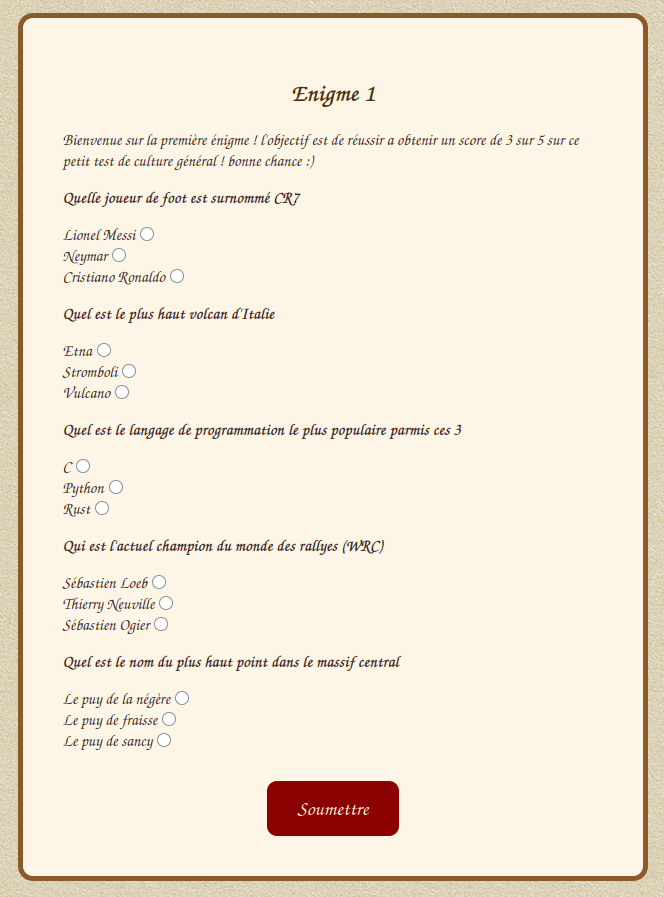
\includegraphics[scale=0.4]{enigme1.png}

\newpage
\subsection{Enigme 2}
La seconde énigme est un test de rapidité et d'agilité avec la souris. Un lien sous forme de bouton rouge va apparaître à un endroit au hasard à l'écran, vous devez cliquer dessus le plus rapidement possible avant d'être rediriger de force vers la page du début de l'énigme! Cliquez avec succès sur 10 boutons, et vous pourrez accéder à l'énigme suivante. Vous disposez de 3 secondes pour cliquez sur le premier bouton, et pour chque bouton sur lesquels vous cliquez, le chrono diminue de 0.2 secondes, pour un temps de seulement 1 seconde à la fin! \\

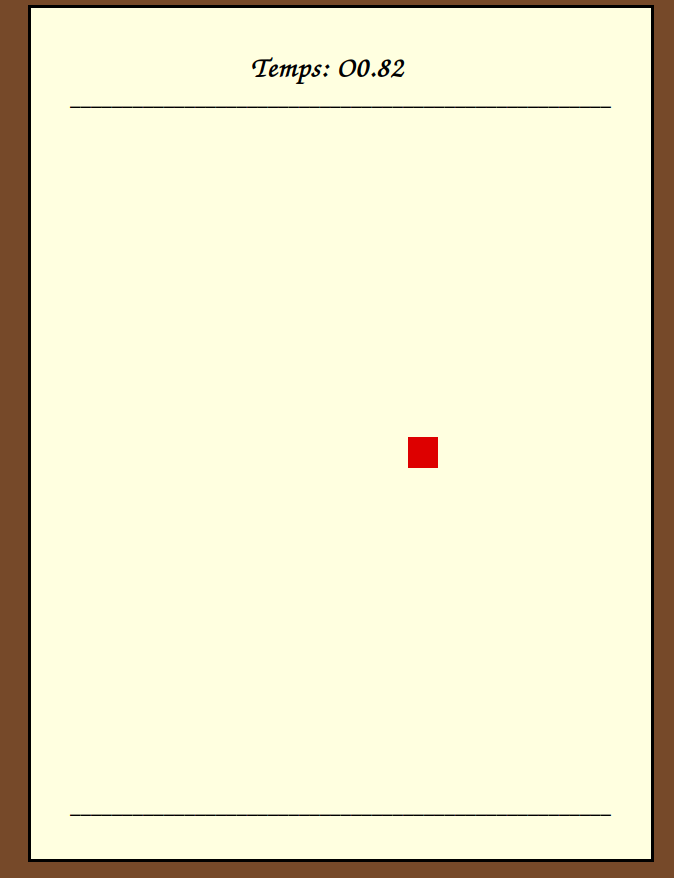
\includegraphics[scale=0.45]{enigme2.png}

\newpage
\subsection{Enigme 3}
La troisième et avant dernière énigme vous prospose un test de mémoire courte, plusieurs mots vont être affichés à l'écran, c'est à vous de mémoriser le plus de détails possibles sur cette page en 20 secondes! Ensuite, une question vous sera posée, répondez bien ou vou serez redirigé au début de l'énigme! L'énigme est composée de 3 niveaux différents, tous plus dur les uns que les autres. Les mots affichés disposent également d'une chance de 1/1000 d'être un lien amenant sur une page secrète, inutile, mais secrète! \\

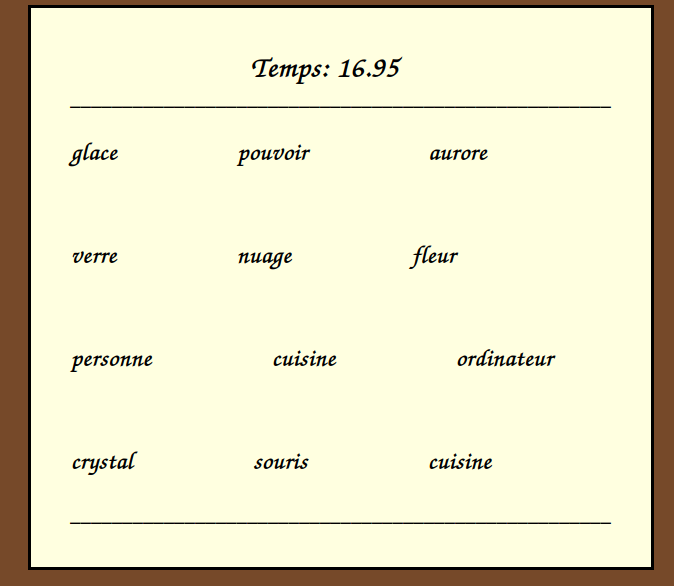
\includegraphics[scale=0.45]{enigme3.png}

\newpage
\subsection{Enigme 4}
La quatrième et dernière énigme est une vraie énigme. Vous devez trouver un code avec des carrés de couleurs affichant des chiffres lorsque vous y passer votre souris. Dans la première page, on vous met en garde: Un bug étrange se produit dans cette énigme. Vous devrez trouver un moyen de le contourner pour arriver à la page finale et compléter la chasse au trésor, bonne chance! \\

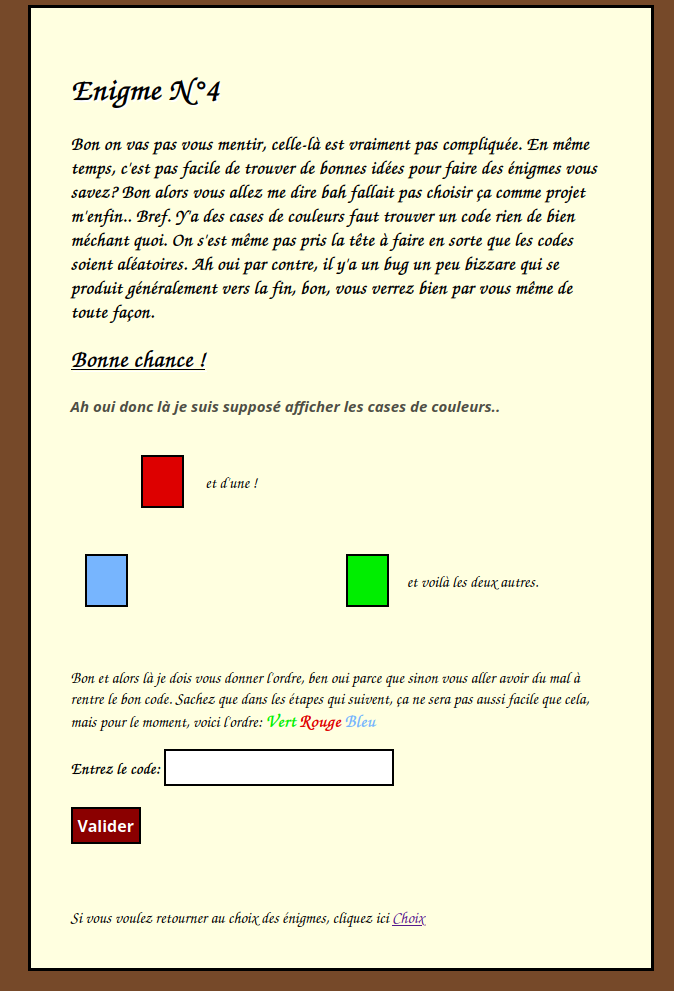
\includegraphics[scale=0.4]{enigme4.png}

\newpage
\section{Autres}
\subsection{Base De Données}
La base de données utilisée dans notre projet est asser simple, elle est composé d'une seule table joueurs avec 4 champs différents:
\begin{itemize}
\item pseudo: sert d'identifiant utilisateur
\item mdp: le mot de passe de l'utilisateur, utilisé pour se connecter
\item progres: le progres de l'utilisateur dans la chasse, varie de 1 à 5
\item: statut: statut d'admin ou non, les admins ont accès à toutes les énigmes lorsqu'il se connectent
\end{itemize}

\subsection{Répartition du travail}
Le travail a été réparti équitablement entre les membres du groupe, chacun y a fait ça part. ChatGPT et autres IA génératives de texte n'ont pas été utilisées pour ce projet.
  

\end{document}